\documentclass{beamer}
\usetheme{Boadilla}

\usepackage[english]{babel}
\usepackage[T1]{fontenc}
\usepackage[latin1]{inputenc}
\usepackage{tikz}
\usepackage{verbatim}
\usepackage{animate}
\usepackage{calc}
\usepackage{fp}
\usepackage{times}

\newcommand\layera{%
\path (0,0) node[circle,minimum size=15pt,draw] (00) {0};
}

\newcommand\layerb{%
\path (-1,-1) node[circle,minimum size=15pt,draw] (111){};
\draw[->] (00) -- (111);
}


\title[MUMmer]{Alignment of whole genomes using MUMmer}

\subtitle{Presentation in Algorithms in Bioinformatics (T�111F autumn 2014)}

\author{Hannes P�tur Eggertsson}

\date{November 18, 2014}

%\setbeamertemplate{frametitle}[default][center]


\begin{document}

\begin{frame}[plain]
\titlepage
\end{frame}

%%%%%%%%%%%%%%%%%%%%%%%%%%%%%%%%%%%%%%%%%%%%%%%%%%%%%%%%%%%%%%%%

%\begin{frame}{Motivation}
%Let's go back to 1999... (some things that will remind you of that wonderful time)
%
%{
%	
\includegraphics[width=0.3\textwidth]{img/Win98.png}<2-4>
%	
\includegraphics[width=0.35\textwidth]{img/blue.png}<3-4>
%	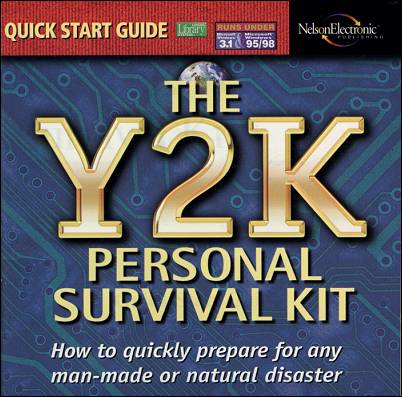
\includegraphics[width=0.34\textwidth]{img/y2k.jpg}<4>
%}
%\end{frame}

\begin{frame}{Motivation}
In 1999...
\begin{itemize}
\item the number of sequenced genomes was increasing rapidly
\item when a new genome is sequenced, one could ask himself:
\begin{itemize}
\item How does this genome align to the other genomes?
\end{itemize}
\end{itemize}

Problem: 
\begin{itemize}
\item We have algorithms that were used for single gene sequences (up to 10,000 bp)
\item But, they won't work well with whole genomes (millions of base pairs or more)
\begin{itemize}
\item Take up way too much memory or
\item Have unacceptable computational time
\end{itemize}
\end{itemize}
\end{frame}

\begin{frame}{Introduction}
%	{ 
%		\includegraphics[width=0.6\textwidth]{img/turmite.png}
%	}
MUMmer:
\begin{itemize}
\item Is a system used to align whole genome sequences.
\item Uses suffix trees as a data structure.
\item Assumes that the two genomes are similar/related.
\item The algorithm can be split into several steps that I'll talk about in detail
\end{itemize}
\end{frame}

%\begin{frame}{MUMmer}
%Five steps:
%\begin{enumerate}
%\item Creates a suffix tree
%\item Perform a maxumal unique match (MUM) decomposition of two genomes
%\item Sorts the matches found in the MUM alignment
%\item ....
%\end{enumerate}
%\end{frame}

\begin{frame}{Step 1: Creating a suffix tree}
A suffix tree is a compact representation that stores all possible suffixes of an input sequence.
\begin{itemize}
\item Square nodes are leaves.
\begin{itemize}
\item Store information about the starting position of the suffix.
\end{itemize} 
\item Circular nodes are internal nodes.
\begin{itemize}
\item That means two or more sequences share the same prefix.
\item Store information about the length of the shared prefix.
\end{itemize}
\end{itemize}
\begin{center}
	{
		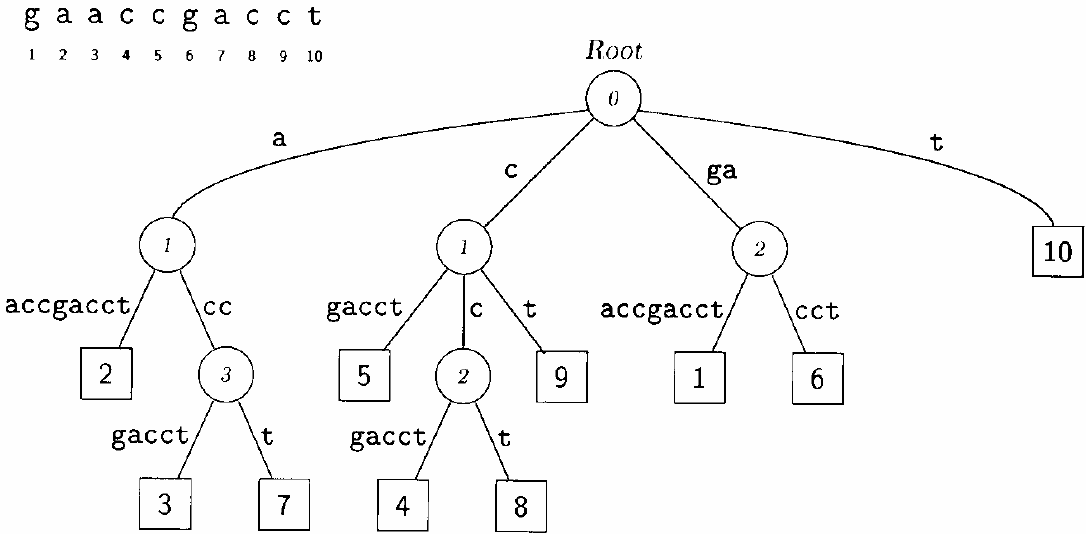
\includegraphics[width=0.65\textwidth]{img/suffixTree.png}
	}
\end{center}
\end{frame}

\begin{frame}{Step 1: Creating a suffix tree}

\only<1>{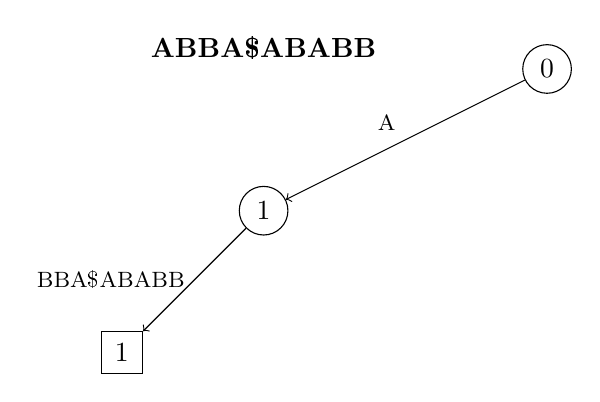
\begin{tikzpicture}[scale=1.8]<1>
\draw (-2,0) node[above] {\textbf{ABBA\$ABABB}};
\path (0,0) node[circle,minimum size=15pt,draw] (00) {0};

\path (-2,-1) node[circle,minimum size=15pt,draw] (121){1};
\draw[->] (00) -- node[above left]{\footnotesize A} (121);
\path (-3,-2) node[rectangle,minimum size=15pt,draw] (122){1};
\draw[->] (121) -- node[left]{\footnotesize BBA\$ABABB} (122);
\end{tikzpicture}}

\only<2>{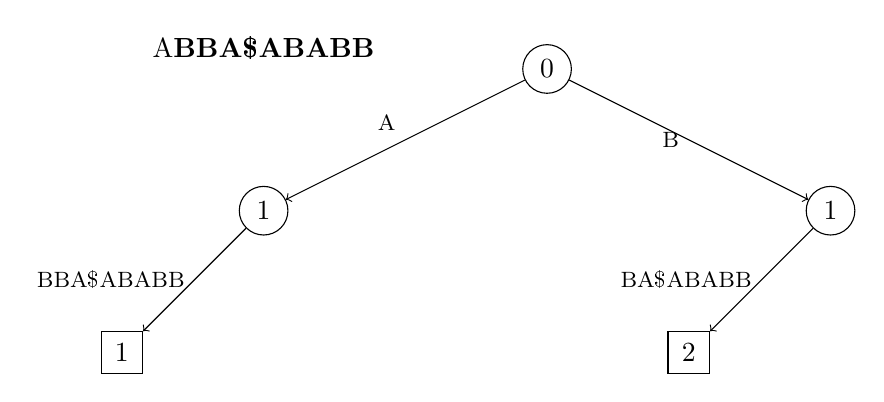
\begin{tikzpicture}[scale=1.8]<1>
\draw (-2,0) node[above] {A\textbf{BBA\$ABABB}};
\path (0,0) node[circle,minimum size=15pt,draw] (00) {0};

\path (-2,-1) node[circle,minimum size=15pt,draw] (121){1};
\draw[->] (00) -- node[above left]{\footnotesize A} (121);
\path (-3,-2) node[rectangle,minimum size=15pt,draw] (122){1};
\draw[->] (121) -- node[left]{\footnotesize BBA\$ABABB} (122);

\path (2,-1) node[circle,minimum size=15pt,draw] (01){1};
\draw[->] (00) -- node[left]{\footnotesize B} (01);
\path (1,-2) node[rectangle,minimum size=15pt,draw] (112){2};
\draw[->] (01) -- node[left]{\footnotesize BA\$ABABB} (112);
\end{tikzpicture}}

\only<3>{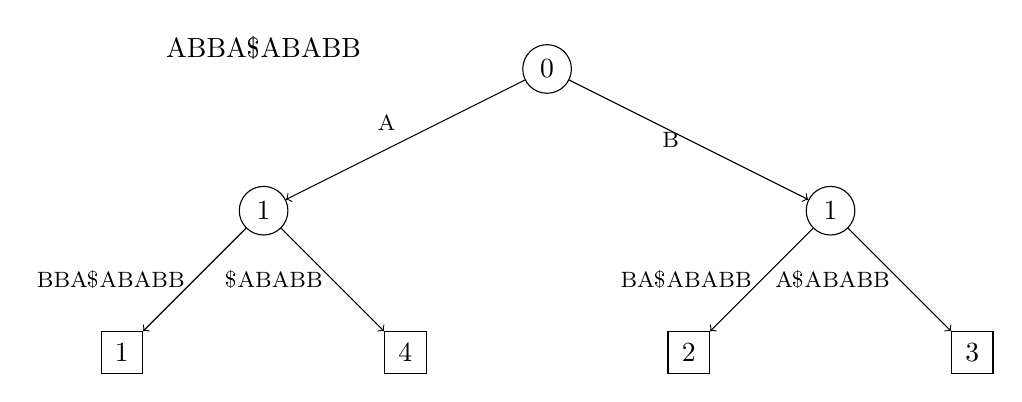
\begin{tikzpicture}[scale=1.8]<1>
\draw (-2,0) node[above] {ABBA\$ABABB};
\path (0,0) node[circle,minimum size=15pt,draw] (00) {0};
% \newframe
\path (-2,-1) node[circle,minimum size=15pt,draw] (121){1};
\draw[->] (00) -- node[above left]{\footnotesize A} (121);
\path (-3,-2) node[rectangle,minimum size=15pt,draw] (122){1};
\draw[->] (121) -- node[left]{\footnotesize BBA\$ABABB} (122);
% \newframe
\path (2,-1) node[circle,minimum size=15pt,draw] (01){1};
\draw[->] (00) -- node[left]{\footnotesize B} (01);
\path (1,-2) node[rectangle,minimum size=15pt,draw] (112){2};
\draw[->] (01) -- node[left]{\footnotesize BA\$ABABB} (112);
% \nf
\path (3,-2) node[rectangle,minimum size=15pt,draw] (12){3};
\draw[->] (01) -- node[left]{\footnotesize A\$ABABB} (12);
% \nf
\path (-1,-2) node[rectangle,minimum size=15pt,draw] (012){4};
\draw[->] (121) -- node[left]{\footnotesize \$ABABB} (012);
% \nf


\end{tikzpicture}}

\vspace*{2cm}
\textsc{ }
\end{frame}

\begin{frame}{Step 2: MUM decomposition}
Let us first define what a MUM is
\begin{definition}
A subsequence is a MUM (Maximal Unique Matches) if and only if:
\begin{itemize}
\item The subsequence has a exact match on both genomes
\item It is not a subsequence of another matched sequence
\begin{itemize}
\item This means the sequence is surrounded be mismatches
\end{itemize}
\item It is unique
\begin{itemize}
\item It appears exactly once in both genomes
\end{itemize}
\end{itemize}
\end{definition}
\begin{example}
\texttt{tcgatcGACGATCGCGGCCGTAGATCGAATAACGAGAGAGCATAAcgactta}
\texttt{gcattaGACGATCGCGGCCGTAGATCGAATAACGAGAGAGCATAAtccagag}
\end{example}

\end{frame}

\begin{frame}{Step 3: Sorting the matches found in the MUM alignment}
Once we have found the MUMs, we might end up with something like this:

{
	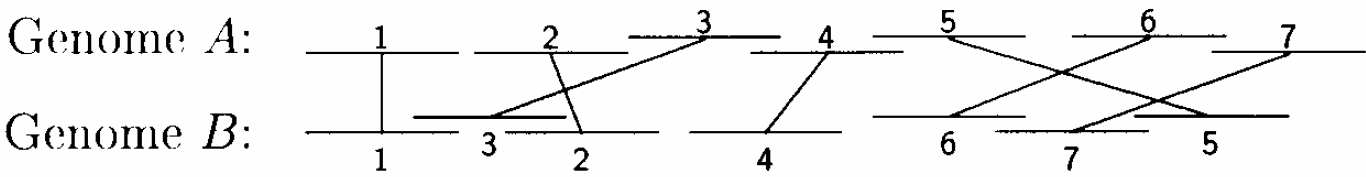
\includegraphics[width=0.75\textwidth]{img/sort1.png}
}

Problem! We cannot align the two genomes using the MUMs because they aren't in correct order.
\end{frame}

\begin{frame}{Step 4: Closing the gaps}

\end{frame}

\begin{frame}{MUMmer 3}

\end{frame}


\begin{frame}{Conclusion}

\end{frame}

\end{document}
